\chapter{Aufbau}
\section{Versuchsaufbau}
Das folgende Bild zeigt unseren Versuchsaufbau während dem ersten Teil der Messung.
\begin{figure}[h]
    \centering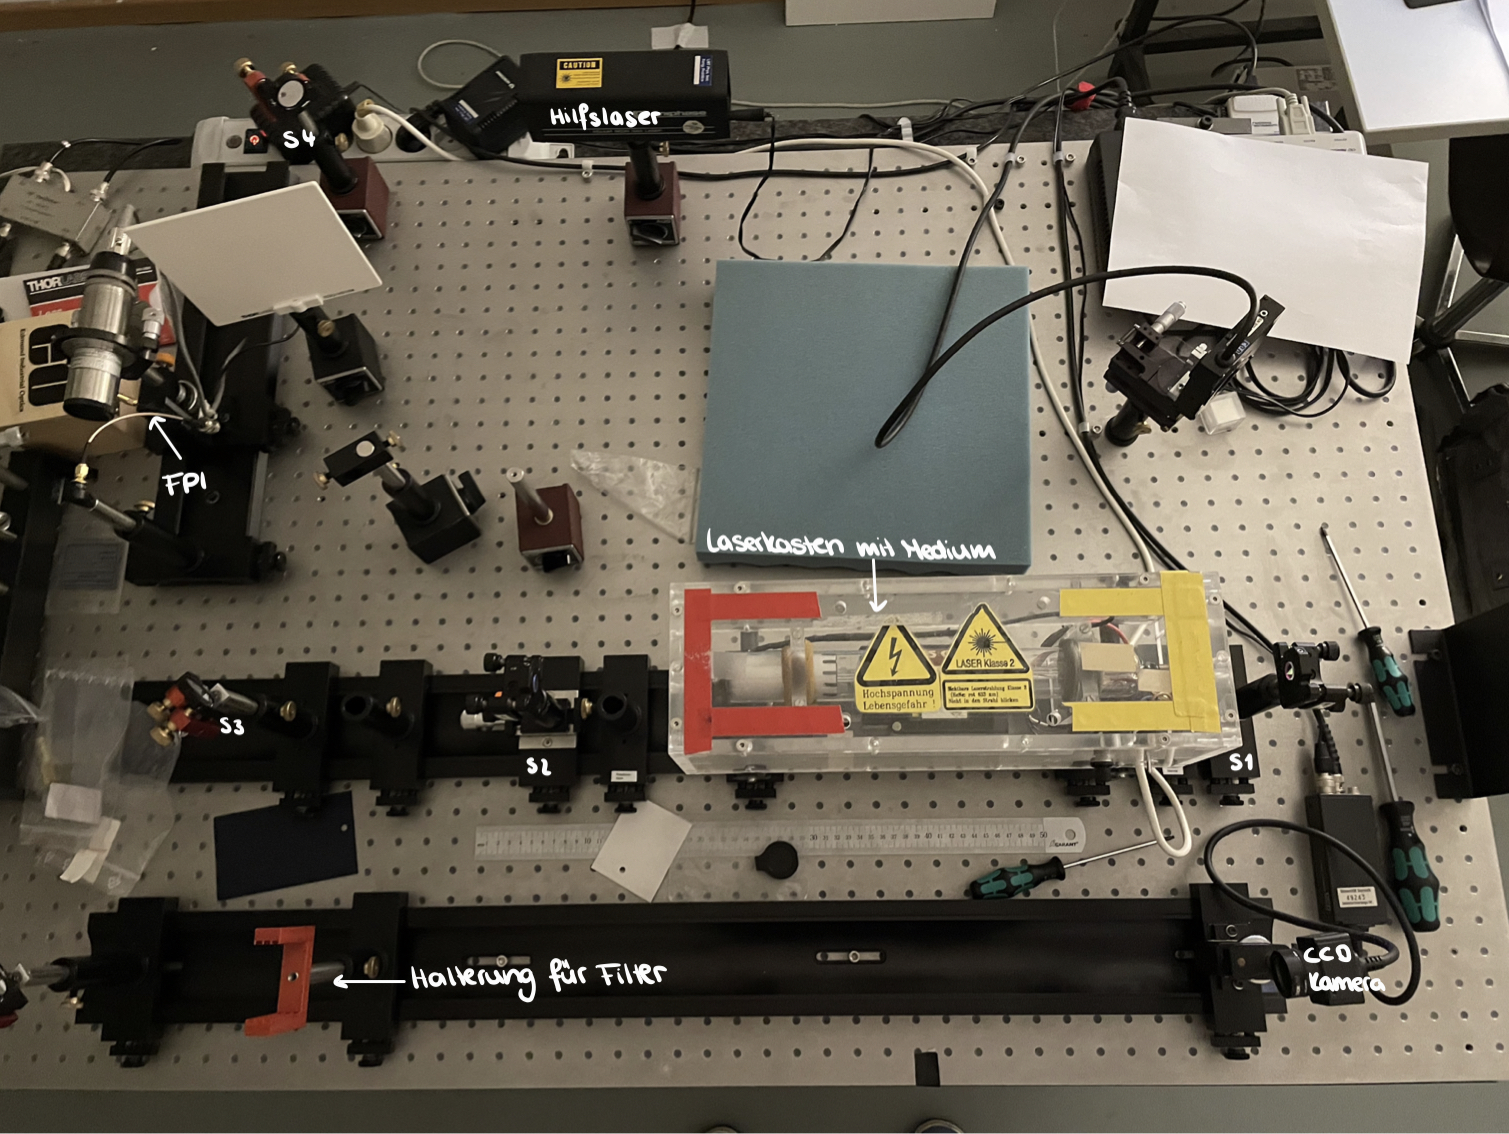
\includegraphics[scale=0.2]{Bilder/Aufbau.jpeg} 
    \caption{Foto des Versuchsaufbaus für den ersten Teil des Versuches.} 
    \label{fig:Aufbau}
\end{figure}\\
In diesem Versuch wird eine Helium-Neon-Gasentladungsröhre als aktives Medium verwendet. 
Auf eine optische Bank wird der Laserkasten mit den beiden sphärischen Spiegeln angebracht. 
Beide Spiegel haben einen Krümmungsradius von $500\,mm$. Der hintere Spiegel, in 
dem Foto \ref{fig:Aufbau} als S1 gekennzeichnet, hat 99,9\% Reflektivität und der im Foto 
als S2 markierten Spiegel hat eine Reflektivität von 98\%. 
Damit der Laser stabil läuft muss die folgende Gleichung erfüllt sein:
\begin{equation}
    g_1 \cdot g_2 \leq 1
\end{equation}
wobei $g_i = 1 - \frac{L}{r_i}$ mit L: Spiegelabstand und $r_i$: Krümmungsradius.
Damit ergibt sich, dass die beiden Spiegeln maximal $500\,mm$ voneinander entfernt sein dürfen.\\
Bei uns hatten die Spiegel 1 und Spiegel 2 einen Abstand von: $L = (54,5 \pm 0,2)\,cm$.\\
Bei uns ist die Bedingung nicht exakt erfüllbar gewesen, da es vom Aufbau her nicht möglich war die 
Spiegel näher zueinander zubekommen, da die anderen optischen Geräte, wie beispielweise die 
Lochblende, noch zwischen den Spiegeln angebracht werden musste. \\
Für die anderen Versuchsteile wird das Laserlicht so umgelenkt, das es auf die CCD-Kamera oder auf 
das Fabry-Pérot-Interferometer trifft. \\
Die entsprechenden Längen zwischen den verwendeten Bauelementen sind dem Protokoll, im Anhang, zu entnehmen. 

\section{Justierung}
Bevor die Messung startet, musste der Laser erst noch justiert werden.
Hierzu wird mithilfe eines Hilfslaser und der Lochblende eine optische Achse definiert. 
Zuerst wird die Höhe des Hilfslaserstrahls auf ca. 21,5\,cm eingestellt und dessen Laserstrahl
parallel zur optischen Achse ausgerichtet. 
Anschließend wird der Laserkasten in den Strahlengang eingebracht und so eingestellt, dass 
der Laserstrahl mit einer möglichst hohen Intensität wieder aus dem Medium austritt. 
Dann wird zuerst der total reflektierende Spiegel eingebracht und so justiert bis der 
eintreffende Strahl sich selbst reflektiert. 
Zuletzt wird noch der teil-transmittierender Spiegel angebracht. Auch hier 
wird wieder die Position so lange verändert bis der transmittierte Strahl auf 
den Spiegel trifft. 
Der Hilfslaser wird nun abgeschaltet und das Laseraktive Medium angeschaltet.
Danach wurden die reflektierenden Spiegel leicht verstellt, bis der Laserstrahl angesprungen ist.
Zum Schluss wird noch feinjustiert mithilfe des Powermeter, die Spiegel werden solange 
verändert bis die maximale Intensität erreicht wird. Bei uns liegt der Peak bei 
$P = (4,32 \pm 0,03)\,mW$.




